\section{Анализ предметной области}

\subsection{Проблема прогнозирования ошибок и сбоев устройств}

Эффективная эксплуатация промышленных устройств
требует наличия надежных обслуживающих систем,
которые должны предоставлять безопасные, отказоустойчивые решения,
поэтому предотвращение ошибок и сбоев имеет первостепенное значение.

Обычно, чтобы предотвратить сбои и ошибки, операторы,
как правило, выполняют техническое обслуживание 
на основе рекомендаций производителей, 
и им приходится регулярно проверять критически важные детали,
Для этого требуются опытные специалисты с высоким уровнем квалификации.
Данный процесс очень дорог и трудоемок.
Однако, в последнее время получила свое распространение
парадигма промышленного интернета вещей,
являющаяся часть более общего понятия -- интернета вещей,
которая предоставляет идеи соединения
промышленных устройств и датчиков в единую систему.
Такая система может позволить проводить автоматизированный мониторинг и 
анализ критически важных параметров промышленных устройств,
без участия операторов, для обнаружения и предсказания ошибок и сбоев. \cite{iiot}

Не смотря на то, что парадигма промышленного интернета вещей предоставляет идеи
для создания системы, она не дает описания способов и методов реализации этой системы.
Такое положение обусловлено относительно недавним появлением данной парадигмы,
из-за чего еще не устоялась методология и принципы разработки.

Так как на данный момент нет устоявшихся концепций,
ведутся разработки на основе различных подходов,
при этом учитывается специфика промышленных устройств,
для которых разрабатывается система.

Задача разработки системы промышленного интернета вещей можно разбить на две подзадачи,
каждую из которых можно решать отдельно, однако решение второй подзадачи может зависит от решения первой:

\begin{enumerate}
    \item Разработка подсистемы сбора, обработки и хранения данных с различных устройств;
    \item Разработка подсистемы анализа данных для обнаружения и предсказания ошибок и сбоев.
\end{enumerate}

Решение первой подзадачи может стать основной для решения второй подзадачи,
так как для анализ данных требует наличие готовой среды, в которой
будет происходить анализ.

Если первая подзадача может быть решена проектированием грамотной архитектуры и выбора подходящих инструментов,
то для решения второй задачи необходимо определиться с подходами и методами
получения прогнозов ошибок и сбоев, с учетом особенностей данных.

Можно сказать, что для того, чтобы иметь систему обнаружения и прогнозирования ошибок и сбоев устройств,
нужно решить две поставленные подзадачи. Первая подзадача не является темой данной дипломной работы
и выходит за ее рамки, однако, в работе будет описана с учетом преимуществ и недостатков существующая разработанная система,
в контексте которой будет решаться вторая подзадача.

\subsection{Временные ряды}



Поставленную задачу можно охарактеризовать как задачу анализа временных рядов.

Временные ряды -- серия точек данных, индексированных во временном порядке.
Анализ временных рядов представляет собой совокупность методов анализа данных временных рядов,
которые направлены на выявление значимых паттернов. \cite{box-series}

Временные ряды имеют темпоральную структуру, то есть упорядочены во времени,
тем самым анализ временных рядов отличается от перекрестных исследований,
в которых обычно используется анализ выборки или выборок из генеральной совокупности в определенный момент времени.
Кроме этого, анализ временных рядов отличается от пространственного анализа,
который имеет такую же фиксированную основу как и перекрестные исследования,
например, в пространственном анализе могут анализироваться географические объекты, без учета временной компоненты. \cite{shumway-series}

Существует классификация временных рядов: \cite{zhang-series}

\begin{itemize}
    \item одномерные и многомерные;
    \item стационарные и нестационарные;
    \item линейные и нелинейные.
\end{itemize}

Пусть есть процесс $x_t$, где $t \geq 0$ или $-\infty < t < \infty $.

Одномерные представляют собой временной ряд, которые генерируется на основе одного атрибута,
а многомерный имеет больше одного, другими словами в одномерном случае $x_t$ представляет собой вектор,
а в многомерном $x_t$ определяется как матрица.

Данные временного ряда можно представить в виде $n\times d$ матрицы данных: \cite{zaki}

\begin{equation} \label{data_matrix}
    \textbf{D} = 
    \begin{pmatrix}
    x_{1,1} & x_{1,2} & \cdots & x_{1,d} \\
    x_{2,1} & x_{2,2} & \cdots & x_{2,d} \\
    \vdots  & \vdots  & \ddots & \vdots  \\
    x_{n,1} & x_{n,2} & \cdots & x_{n,d} 
    \end{pmatrix}
\end{equation}

Вектор-строки вида:

\begin{equation}
    \textbf{x}_i = (x_{i,1}, ..., x_{i,d})
\end{equation}

в зависимсоти от предметной области имеют различные названия, например:
сущности, объекты, примеры и т.д.

Вектор-столбцы вида:

\begin{equation}
    \textbf{X}_j = (x_{1,j}, ..., x_{n,j})
\end{equation}

также могут иметь различные названия: атрибуты, свойства, переменные и т.д.

Стационарность определяется через требование равносильности совместных распределений вектора
$(x_{t_1}, ..., x_{t_k})$ и вектора $(x_{t_1+t}, ..., x_{t_k+t})$.
Другими словами, в стационарном временном ряде есть повторяющиеся паттерны,
в отличие от нестационарного. \cite{terence-series}

Линейные модели определяются через свойства линейности параметров временного ряда, например среднего и дисперсии.
Нелинейные модели напротив могут иметь нелинейную структуру, что требует использования
нелинейных методов, например, методов нелинейной регрессии. \cite{douglas-series}

Самыми малоизученными являются нелинейные нестационарные модели. \cite{rao-series}
Примеры реализации системы обнаружения и предсказания ошибок,
основанные на данном типе моделей не были найдены и обсуждаться в данной работе не будут,
так как данная область выходит за рамки темы дипломной работы.

Обозначенную выше подзадачу можно разбить также на два элемента:

\begin{enumerate}
    \item Выявление ошибок, обнаружение аномалий;
    \item Предсказание поведения устройства.
\end{enumerate}

Данные задачи можно решать как отдельно, где для каждой задачи будет использоваться свой метод,
так и совместно через один метод. Каждый вариант будет рассмотрен в существующих примерах.

\subsection{Интеллектуальный анализ данных временных рядов}

Также можно сказать, что поставленная задача обнаружения и предсказания ошибок и сбоев
является задачей интеллектуального анализа данных. Коротко опишем что такое интеллектуальный анализ данных.

Интеллектуальный анализ данных (data mining) 
-- процесс выявления паттернов из больших объемов данных. \cite{han-mining}

Интеллектуальный анализ данных представляет собой междисциплинарную область,
в которой используются методы, идеи и принципы из следующих областей:
статистика, машинное обучение, распознавание образов,
вычислительная нейробиология, базы данных.
Стоит отметить, что данная область является частью более широкой области, 
которая называется выявление (обнаружение) знаний из баз данных (knowledge database discovery).
(zaki)

\begin{figure}[h]
    \center{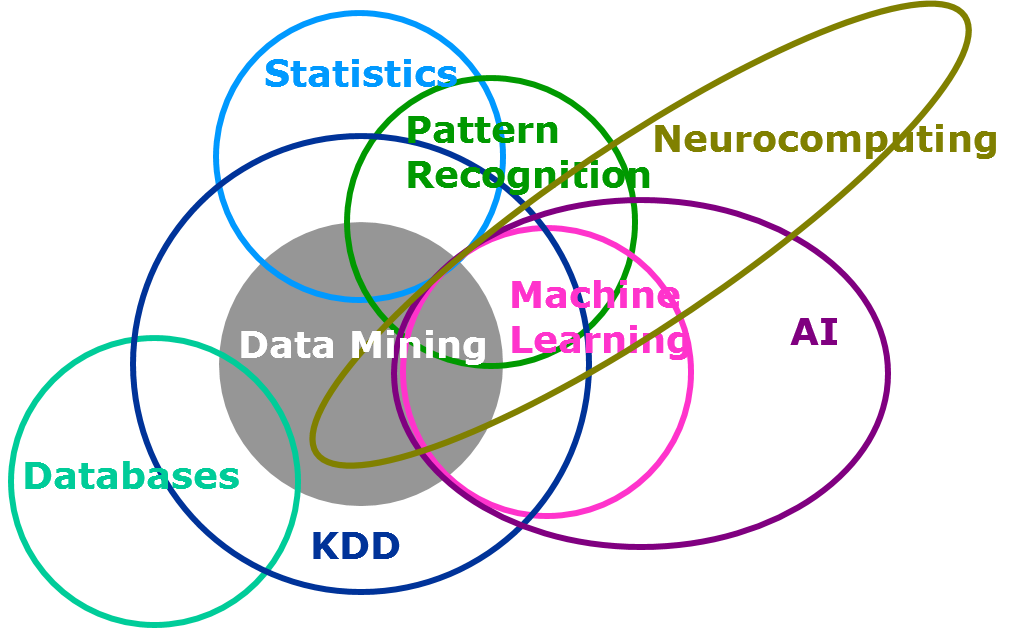
\includegraphics[width=10cm]{img/mining.png}}
    \caption{Место интеллектуального анализа данных среди других областей}
\end{figure}

Кроме этого, интеллектуальный анализ данных можно определить как часть
распознавания образов/паттернов (pattern recognition),
которая связана с обработкой данных из баз данных и выявлением паттернов, 
связанных с определенной предметной областью. \cite{mirkin-mining}
Сама область распознавания образов покрывает и другие области, например,
обработка сигналов и машинное зрение. \cite{mehmed-mining}

Опишем приведенные области, обозначим их основные идеи и принципы.

База данных -- организованная коллекция данных, которая собирается и хранится
при помощи компьютерных систем.
Для взаимодействия пользователя с базой данных используется
система управления базами данных (СУБД).

Теория баз данных поставляет формализованные методы и принципы проектирования и разработки баз данных и СУБД.
Обычно теоретически выделяют два главных типа построения баз данных: реляционные (SQL) и нереляционные базы данных (NoSQL).
Также иногда выделяют смешанный тип, появившейся сравнительно недавно:
новые реляционные базы данных, который совмещает лучшие
идеи и принципы из реляционных и нереляционных теорий и подходов (NewSQL). \cite{fauler-db}

В контексте интеллектуального анализа данных базы данных используются как источник данных.
Сами данные перед анализом обрабатываются, что также является частью процесса обнаружения знаний.
От типа и особенностей сбора и хранения данных в базе зависят последующие шаги анализа данных.



Обнаружение знаний из баз данных (knowledge database discovery, KDD) --  более широкая область
работы с данными из баз данных, частью которой является интеллектуальный анализ данных.
KDD определяют как процесс выявлений знаний (паттернов), который разбит на основные шаги: \cite{curr}

\begin{enumerate}
    \item Селекция -- выборка данных из баз данных по определенным критериям;
    \item Обработка (pre-processing) -- приведение выбранных данных в подходящий вид 
    (очистка и удаление пропущенных значений, фиксирование атрибутов) для последующего анализа;
    \item Трансформация (transformation) -- трансформация данных в подходящую структуру данных, например, в матрицу данных \eqref{data_matrix};
    \item Интеллектуальный анализ данных (data mining) -- обнаружение паттернов в данных;
    \item Интерпретация и оценка (interpretation and evaluation).
\end{enumerate}

Следующим шагом также может быть использование, развертывание и эксплуатация обнаруженных знаний и паттернов для целей предметной области.

Статистика, распознавание образов и машинное обучение являются поставщиками методов для каждого шага процесса KDD.
Каждая из этих областей имеет свои особенности, однако все они имеют также много общего.

\subsection{Существующие решения проблемы}

Итак, рассмотрим существующие решения для обнаружения аномалий, например, ошибок и сбоев в данных, а также
подходы к прогнозированию и оповещению об этом пользователей.


Во-первых, можно сказать, что модели прогнозирования временных рядов, такие как моедль среднего ранга (AR),
модель скользящего среднего (MA), экспоненциальная модель,
модель авторегрессии скользящего среднего (ARMA), 
интегрированная авторегрессионная модель скользящего среднего (ARIMA), 
зависят от параметров, полученных из исторических временных рядов. 
Эти параметры являются неотрицательными целыми числами, 
которые относятся к порядку авторегрессионной части, степени участвующей первой разности и порядку части скользящей средней. 
Хотя эти процессы могут обрабатывать нестационарные данные, 
они ограничены в запоминании любого состояния за любой промежуток времени. \cite{nonlinear-series}

В \cite{3-paper} авторы рассмотрели потоковые данные как частично наблюдаемый Марковский процесс. \cite{3-pomp}
Такое решение было принято с целью создания композиционной системы,
которая состояла из различных моделей: экспоненциальные модели, сезонные модели, модель лог-гауссовского процесса Кокса.
Данная статья содержит хорошие идеи использования фильтров на композиции частично наблюдаемых Марковских процессов, а также
теоретического обоснования такого использования. Однако, хорошая разработанная теория и слабое тестирование на реальных данных
не показало высокой эффективности такого подхода. В данной статье авторы научились только предсказывать аномалии,
но не смогли их определить, а также использовать данный подход в реальном времени.

Федеративное обучение -- один из это методов машинного обучения,
который состоит в обучении алгоритм на нескольких децентрализованных периферийных устройствах или серверах, 
содержащих локальные выборки данных, без обмена их выборками данных.
Использование федеративного обучения для фильтрации данных сети медицинских устройств было рассмотрено в \cite{8-paper}.
Благодаря использованию методов федеративного обучения, авторам удалось повысить энергоэффективность обработки и анализа данных,
то есть решили одну из самых распространенных проблем в сфере интернета вещей.
Также в статье описаны этапы локального анализа данных на самих устройствах и глобального анализа данных на сервере.
Для первого авторы использовали адаптивные фильтры \cite{adaptive-filter}, для второго матричный анализ возмущений \cite{pertuberation}.
Недостатком такого подхода является низкая гибкость, так как может потребоваться использовать корреляционный анализ устройств,
а в распределенном анализе корреляция может быть утрачена, тем самым будут утрачены полезные признаки.
Кроме этого, существуют усовершенствованные адаптивные фильтры, например ядерный рекурсивный фильтр \cite{krls-t}.
Еще можно сказать, что матричный анализ возмущений может не учитывать асинхронную структуру предобработанных данных.
 
В целях мониторинга профиля и обнаружения неисправностей в \cite{4-8} авторы применили модель нелинейной 
параметрической регрессии для разработки системы, которая была бы устойчивой и нечувствительной 
к изменениям температуры в производственной практике. 
В \cite{4-9} был разработан метод мониторинга, который может автоматически адаптировать параметры контрольной карты (метод из теории управления). 
В \cite{4-10} авторы добавили все профили каналов и применили анализ главных компонентов (PCA) 
агрегированным профилям тоннажа для извлечения характеристик. 
В \cite{4-12} использовались как статистические, 
так и вейвлет-характеристики, извлеченные из сигналов датчиков, 
для разработки адаптивного метода обучения для оценки износа инструмента в процессе высокоскоростного фрезерования. 
Каждое из этих исследований было сосредоточено на анализе индивидуального профиля данных, то есть анализ был проведен с одномерными данными.
Однако, выходы датчиков устройства обычно являются многоканальными, что требует многомерного анализа временных рядов.

У многомерных данные могут быть следующие особенности: \cite{wei-series}

\begin{itemize}
    \item С увеличением числа датчиков обработка каждого 
    временного ряда от каждого датчика становится как более интенсивной, что сказывается на повышении вычислительной нагрузки;
    \item Данные имеют больше выбросов и шумов, по сравнению с одномерными данными;
    \item Временные ряды от разных датчиков имеют корреляции на разных уровнях, 
    что приводит к большому количеству избыточной информации, однако необходимо учитывать возможные корреляции;
    \item Состояния работы до простоя обычно продолжаются в течение некоторого времени и включают состояния отказа оборудования. 
    Кроме того, после восстановления неисправного датчика также появляется период задержки в рабочем состоянии. 
    Следовательно, модель прогнозирования должна иметь инвариантность памяти относительно таких состояний. 
\end{itemize}


Эти особенности данных приводят к следующим вопросам исследования:

\begin{itemize}
    \item Как уменьшить избыточную информацию без ухудшения точности прогнозирования?
    \item Как определить выбросы и шумы?
    \item Как моделировать долгую память состояний?
    \item Как точно предсказать текущее состояние на основе исторических данных?
\end{itemize}

Опишем существующие результаты, которые отвечают на эти вопросы.

(примеры использования многомерного анализа, нейронных сетей, обучения с подкреплением, а также анализ преимуществ и недостатков этих примеров)

\subsection{Определение решаемых задач}

Окончательно определим задачи, которые необходимо решить.

Перед анализом данные сами данные сначала необходимо подготовить.
Для этого база данных должна иметь исправную схему данных с правильными параметрами.
Также, стоит взять часть данных для последующего анализа.

Для решения проблемы выявления паттернов и аномалий необходимо выбрать наилучшую модель кластеризации,
а также протестировать ее, обосновать ее выбор и интегрировать с учетом особенностей обучения на потоковых данных в реальном времени.

Следующей задачей, которую необходимо решить, является выбор предсказательной модели и обоснование данного выбора.
Данную модель также необходимо протестировать, а потом интегрировать с моделью кластеризации.

Заключительным этапом является внедрение в эксплуатацию разработанной подсистемы выявления и предсказания ошибок и сбоев на станках лазерной резки.


\subsection{Выводы}

В данной главе была обозначена проблема выявления ошибок и сбоев на станках лазерной резки и в устройствах вообще.
Были описаны особенности данной проблемы, а также ее теоретические аспекты. Кроме этого, был проведен анализ
существующих решений, базирующихся на различных методах, подходах и идеях.
Для каждого случая была дана критика, а именно обозначены достоинства и недостатки каждого решения.

В конце главы были обозначены задачи, решения которых может помочь достичь решения проблемы выявления ошибок и прогнозирования.

\clearpage